\section{Memory hierarchy}

Since 1980, there has been a notable divergence in performance between CPUs and DRAM.
To bridge this gap, architects introduced small, high-speed cache memories between the CPU and DRAM, establishing a memory hierarchy.

During the period from 1980 to 1986, DRAM latency decreased by 9\% annually, while CPU performance saw a steady increase of 1.35 times per year.
Post-1986, CPU performance accelerated further to 1.55 times per year, while DRAM performance remained relatively constant.

With the advent of recent multicore processors, the design of memory hierarchy has become increasingly critical.
\begin{example}
    Consider the Intel Core i7 processor, which boasts the capability to generate two references per core clock cycle. 
    With a total of four cores operating at a clock frequency of $3.2\:GHz$, it can achieve a good throughput.
    Specifically, it can handle 25.6 billion 64-bit data references per second and 12.8 billion 128-bit instruction references per second, resulting in a combined throughput of $409.6\:GB/s$.
    However, this remarkable processing power highlights a contrast with the DRAM bandwidth, which is merely 6\% of the total throughput, amounting to a modest $25\:GB/s$.
\end{example}
To address this challenge, several solutions are necessary:
\begin{itemize}
    \item Implementation of multi-port, pipelined caches to enhance data access efficiency.
    \item Adoption of a two-level cache structure per core to optimize data retrieval.
    \item Integration of a shared third-level cache directly on the chip to further streamline memory access.
\end{itemize}
In modern high-end microprocessors, the on-chip cache capacity has surpassed 10 MB, albeit at the cost of significant area and power consumption.

The ultimate goal of memory hierarchy is to create the illusion of a vast, speedy, and cost-effective memory system that allows programs to access a memory space scalable to the size of the disk, with speeds comparable to register access.
Achieving this necessitates the establishment of a memory hierarchy comprising various technologies, costs, and sizes, each with distinct access mechanisms.
\begin{figure}[H]
    \centering
    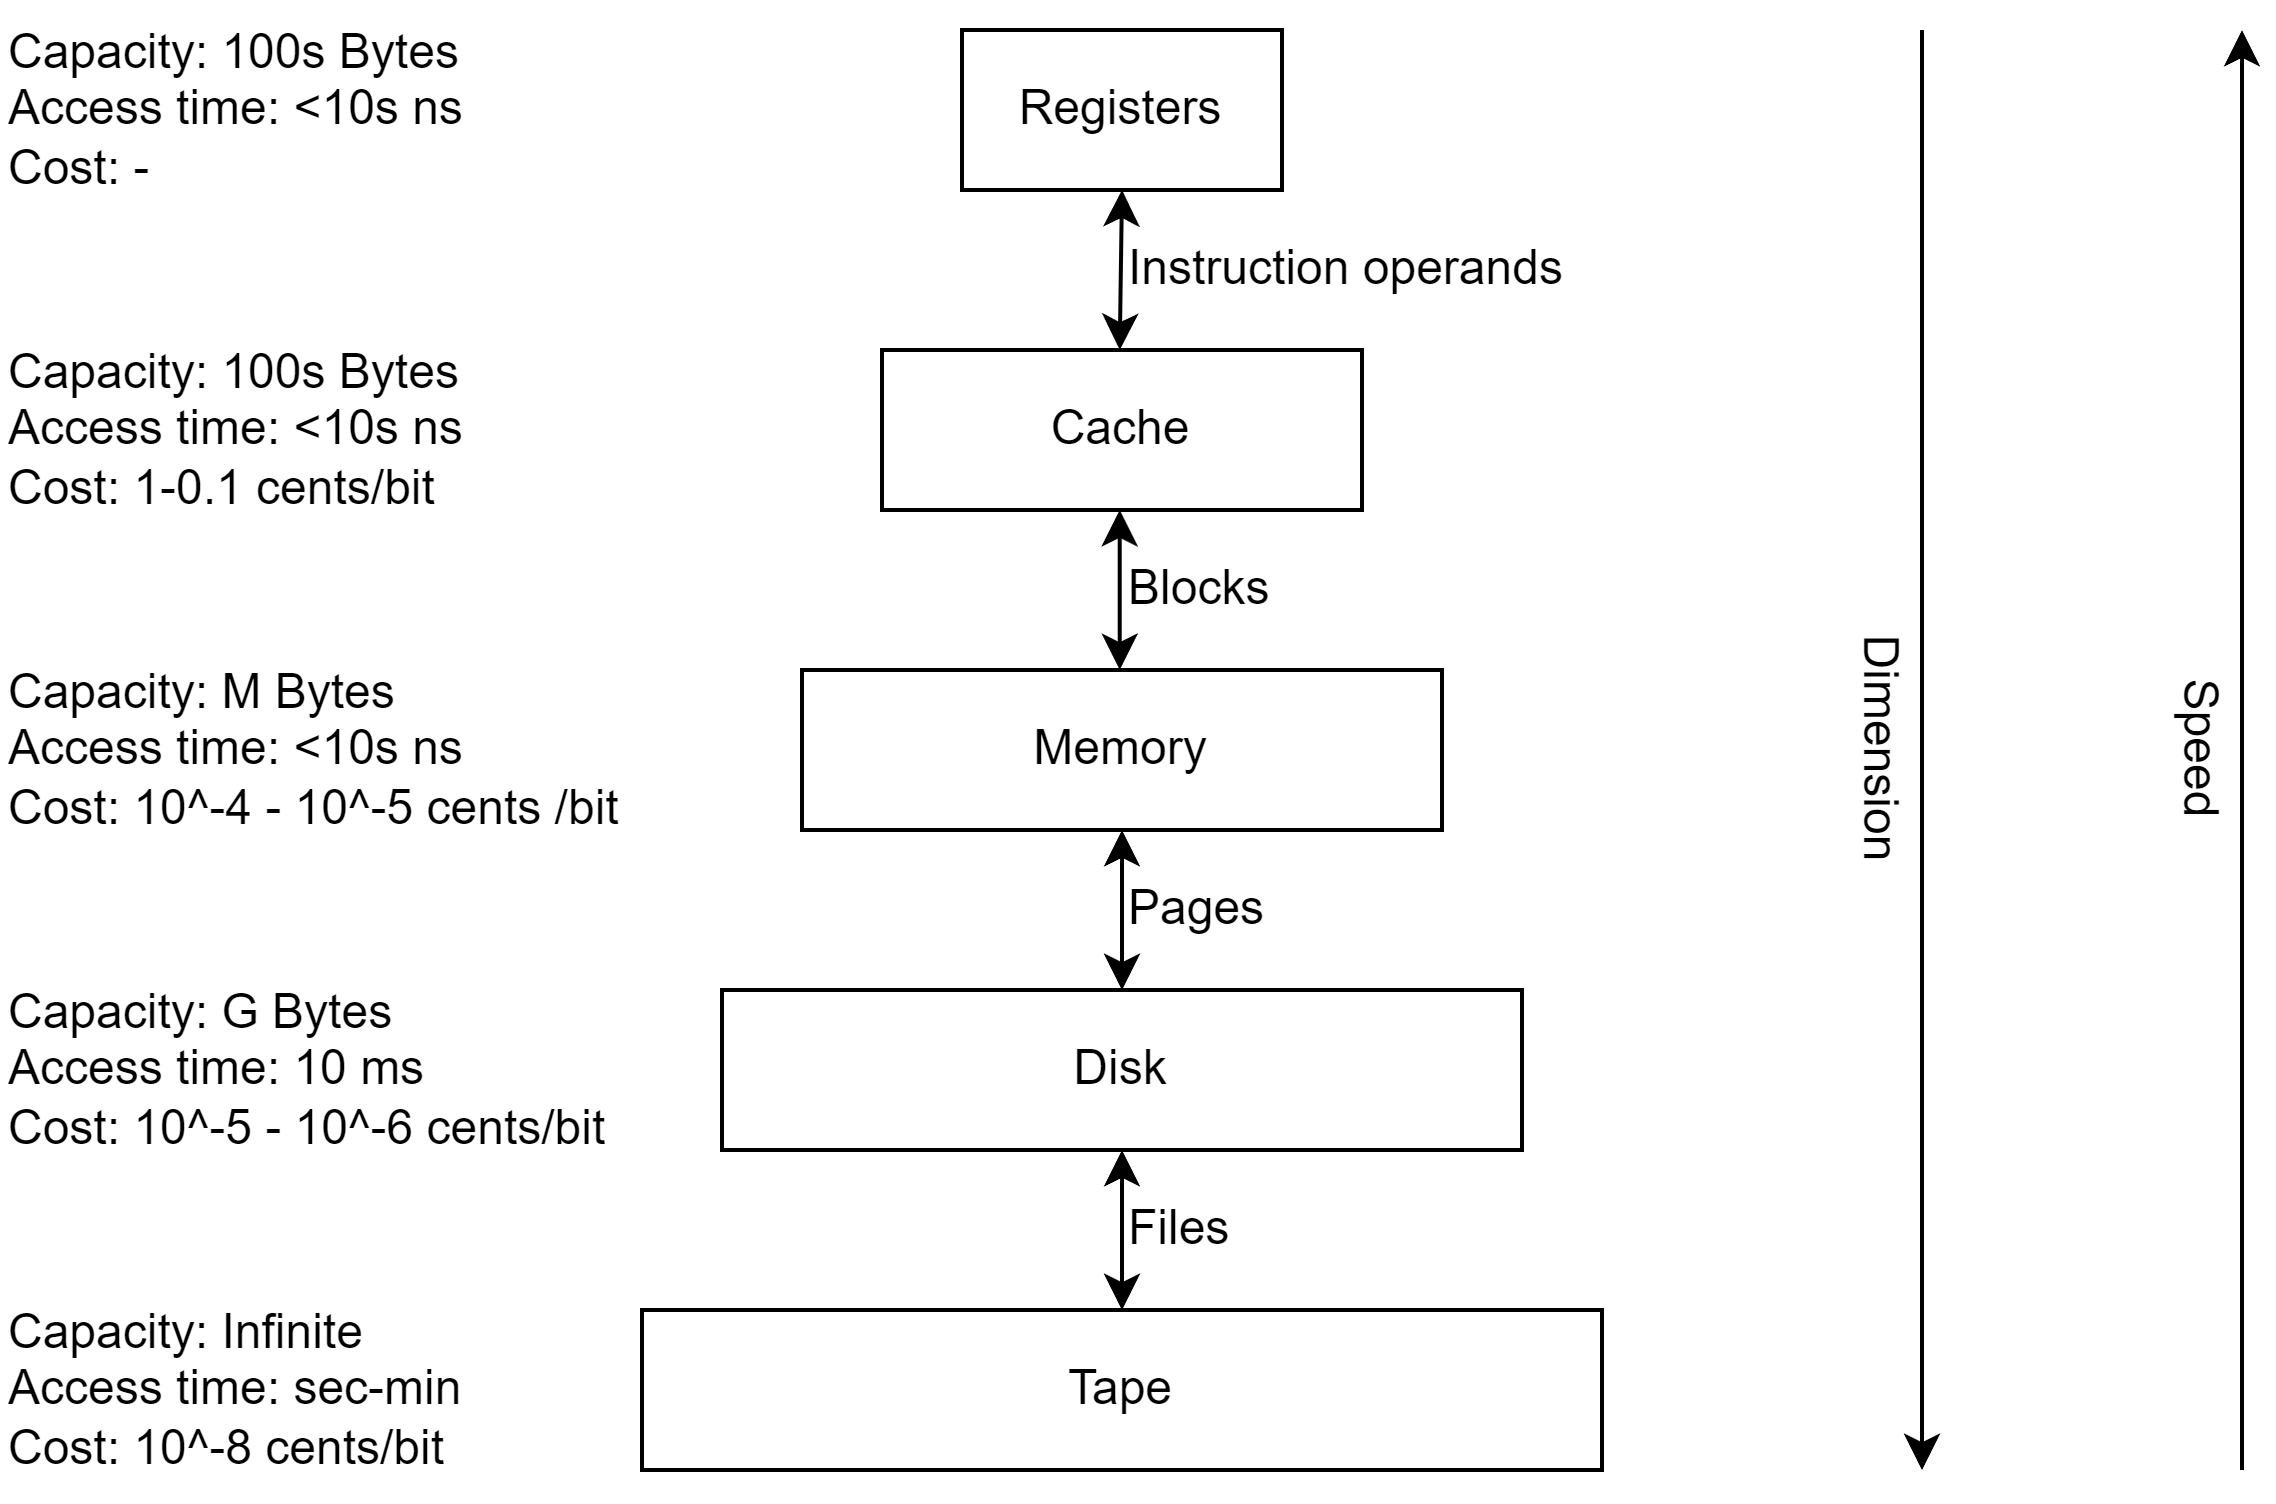
\includegraphics[width=0.75\linewidth]{images/hierarchy.png}
    \caption{Memory hierarchy}
\end{figure}